% Options for packages loaded elsewhere
\PassOptionsToPackage{unicode}{hyperref}
\PassOptionsToPackage{hyphens}{url}
%
\documentclass[
  a5paper,
  landscape,
  notitlepage]{report}
\usepackage{amsmath,amssymb}
\usepackage{lmodern}
\usepackage{ifxetex,ifluatex}
\ifnum 0\ifxetex 1\fi\ifluatex 1\fi=0 % if pdftex
  \usepackage[T1]{fontenc}
  \usepackage[utf8]{inputenc}
  \usepackage{textcomp} % provide euro and other symbols
\else % if luatex or xetex
  \usepackage{unicode-math}
  \defaultfontfeatures{Scale=MatchLowercase}
  \defaultfontfeatures[\rmfamily]{Ligatures=TeX,Scale=1}
  \setmainfont[]{MS Gothic}
  \setmonofont[]{MS Gothic}
\fi
% Use upquote if available, for straight quotes in verbatim environments
\IfFileExists{upquote.sty}{\usepackage{upquote}}{}
\IfFileExists{microtype.sty}{% use microtype if available
  \usepackage[]{microtype}
  \UseMicrotypeSet[protrusion]{basicmath} % disable protrusion for tt fonts
}{}
\makeatletter
\@ifundefined{KOMAClassName}{% if non-KOMA class
  \IfFileExists{parskip.sty}{%
    \usepackage{parskip}
  }{% else
    \setlength{\parindent}{0pt}
    \setlength{\parskip}{6pt plus 2pt minus 1pt}}
}{% if KOMA class
  \KOMAoptions{parskip=half}}
\makeatother
\usepackage{xcolor}
\IfFileExists{xurl.sty}{\usepackage{xurl}}{} % add URL line breaks if available
\IfFileExists{bookmark.sty}{\usepackage{bookmark}}{\usepackage{hyperref}}
\hypersetup{
  hidelinks,
  pdfcreator={LaTeX via pandoc}}
\urlstyle{same} % disable monospaced font for URLs
\usepackage[margin=5mm]{geometry}
\usepackage{color}
\usepackage{fancyvrb}
\newcommand{\VerbBar}{|}
\newcommand{\VERB}{\Verb[commandchars=\\\{\}]}
\DefineVerbatimEnvironment{Highlighting}{Verbatim}{commandchars=\\\{\}}
% Add ',fontsize=\small' for more characters per line
\usepackage{framed}
\definecolor{shadecolor}{RGB}{248,248,248}
\newenvironment{Shaded}{\begin{snugshade}}{\end{snugshade}}
\newcommand{\AlertTok}[1]{\textcolor[rgb]{0.94,0.16,0.16}{#1}}
\newcommand{\AnnotationTok}[1]{\textcolor[rgb]{0.56,0.35,0.01}{\textbf{\textit{#1}}}}
\newcommand{\AttributeTok}[1]{\textcolor[rgb]{0.77,0.63,0.00}{#1}}
\newcommand{\BaseNTok}[1]{\textcolor[rgb]{0.00,0.00,0.81}{#1}}
\newcommand{\BuiltInTok}[1]{#1}
\newcommand{\CharTok}[1]{\textcolor[rgb]{0.31,0.60,0.02}{#1}}
\newcommand{\CommentTok}[1]{\textcolor[rgb]{0.56,0.35,0.01}{\textit{#1}}}
\newcommand{\CommentVarTok}[1]{\textcolor[rgb]{0.56,0.35,0.01}{\textbf{\textit{#1}}}}
\newcommand{\ConstantTok}[1]{\textcolor[rgb]{0.00,0.00,0.00}{#1}}
\newcommand{\ControlFlowTok}[1]{\textcolor[rgb]{0.13,0.29,0.53}{\textbf{#1}}}
\newcommand{\DataTypeTok}[1]{\textcolor[rgb]{0.13,0.29,0.53}{#1}}
\newcommand{\DecValTok}[1]{\textcolor[rgb]{0.00,0.00,0.81}{#1}}
\newcommand{\DocumentationTok}[1]{\textcolor[rgb]{0.56,0.35,0.01}{\textbf{\textit{#1}}}}
\newcommand{\ErrorTok}[1]{\textcolor[rgb]{0.64,0.00,0.00}{\textbf{#1}}}
\newcommand{\ExtensionTok}[1]{#1}
\newcommand{\FloatTok}[1]{\textcolor[rgb]{0.00,0.00,0.81}{#1}}
\newcommand{\FunctionTok}[1]{\textcolor[rgb]{0.00,0.00,0.00}{#1}}
\newcommand{\ImportTok}[1]{#1}
\newcommand{\InformationTok}[1]{\textcolor[rgb]{0.56,0.35,0.01}{\textbf{\textit{#1}}}}
\newcommand{\KeywordTok}[1]{\textcolor[rgb]{0.13,0.29,0.53}{\textbf{#1}}}
\newcommand{\NormalTok}[1]{#1}
\newcommand{\OperatorTok}[1]{\textcolor[rgb]{0.81,0.36,0.00}{\textbf{#1}}}
\newcommand{\OtherTok}[1]{\textcolor[rgb]{0.56,0.35,0.01}{#1}}
\newcommand{\PreprocessorTok}[1]{\textcolor[rgb]{0.56,0.35,0.01}{\textit{#1}}}
\newcommand{\RegionMarkerTok}[1]{#1}
\newcommand{\SpecialCharTok}[1]{\textcolor[rgb]{0.00,0.00,0.00}{#1}}
\newcommand{\SpecialStringTok}[1]{\textcolor[rgb]{0.31,0.60,0.02}{#1}}
\newcommand{\StringTok}[1]{\textcolor[rgb]{0.31,0.60,0.02}{#1}}
\newcommand{\VariableTok}[1]{\textcolor[rgb]{0.00,0.00,0.00}{#1}}
\newcommand{\VerbatimStringTok}[1]{\textcolor[rgb]{0.31,0.60,0.02}{#1}}
\newcommand{\WarningTok}[1]{\textcolor[rgb]{0.56,0.35,0.01}{\textbf{\textit{#1}}}}
\usepackage{longtable,booktabs,array}
\usepackage{calc} % for calculating minipage widths
% Correct order of tables after \paragraph or \subparagraph
\usepackage{etoolbox}
\makeatletter
\patchcmd\longtable{\par}{\if@noskipsec\mbox{}\fi\par}{}{}
\makeatother
% Allow footnotes in longtable head/foot
\IfFileExists{footnotehyper.sty}{\usepackage{footnotehyper}}{\usepackage{footnote}}
\makesavenoteenv{longtable}
\usepackage{graphicx}
\makeatletter
\def\maxwidth{\ifdim\Gin@nat@width>\linewidth\linewidth\else\Gin@nat@width\fi}
\def\maxheight{\ifdim\Gin@nat@height>\textheight\textheight\else\Gin@nat@height\fi}
\makeatother
% Scale images if necessary, so that they will not overflow the page
% margins by default, and it is still possible to overwrite the defaults
% using explicit options in \includegraphics[width, height, ...]{}
\setkeys{Gin}{width=\maxwidth,height=\maxheight,keepaspectratio}
% Set default figure placement to htbp
\makeatletter
\def\fps@figure{htbp}
\makeatother
\setlength{\emergencystretch}{3em} % prevent overfull lines
\providecommand{\tightlist}{%
  \setlength{\itemsep}{0pt}\setlength{\parskip}{0pt}}
\setcounter{secnumdepth}{-\maxdimen} % remove section numbering
\ifluatex
  \usepackage{selnolig}  % disable illegal ligatures
\fi

\author{}
\date{\vspace{-2.5em}}

\begin{document}

\center

\fontsize{34pt}{34pt}\selectfont
\vspace{20pt}

維管束植物和名チェックリストを\\
Rで利用するパッケージwameicheckr\\
(改訂版)

\vspace{15pt}
\fontsize{22pt}{22pt}\selectfont

松村俊和(甲南女子大)

\vspace{20pt}

\begin{itemize}
\tightlist
\item
  和名・学名の問題\\
\item
  よく使われる文献\\
  -- 情報源:Ylist,日本の野生植物,\ldots{}\\
\item
  維管束植物和名チェックリスト,変換シート\\
\item
  解析手順の問題\\
\item
  wameicheckr\\
  -- 特徴,使用方法,注意点・お願い
\item
  類似和名・学名検索(新機能)\\
\item
  その他\\
  -- インストール方法,参考文献
\end{itemize}

\newpage
\fontsize{32pt}{32pt}\selectfont

\begin{center}
和名・学名の問題
\end{center}

\begin{itemize}
\tightlist
\item
  どの文献に従うか?\\
\item
  学名表記の揺れ:結構ややこしい\\
\item
  そもそもの分類の問題もある
\end{itemize}

\begin{center}
\downarrow   
\end{center}

\begin{center}
実際には
\end{center}

\begin{itemize}
\tightlist
\item
  よく使われているもの\\
\item
  便利なもの
\end{itemize}

\newpage

\fontsize{32pt}{32pt}\selectfont

\begin{center}
植生学会誌   

\fontsize{22pt}{22pt}\selectfont
vol.35以降の論文での和名・学名   

\end{center}

\fontsize{28pt}{28pt}\selectfont
\vspace{20pt}

\begin{longtable}[]{@{}ccc@{}}
\toprule
和名・学名の根拠 & 論文数 & うちRを使用 \\
\midrule
\endhead
Ylist & 17 & 9 \\
日本の野生植物 & 3 & 0 \\
Green List & 1 & 1 \\
その他 & 2 & 1 \\
記載なし & 10 & 5 \\
計 & 33 & 16 \\
\bottomrule
\end{longtable}

\newpage

\fontsize{32pt}{32pt}\selectfont

\begin{center}
よく使われる文献
\end{center}

\begin{itemize}
\tightlist
\item
  ネットで入手可\\
  -- Ylist(YL)\\
  -- GreenList(GL)\\
\item
  手入力?\\
  -- 日本の野生植物(WF)
\end{itemize}

\begin{center}
\downarrow   
\end{center}

全てを含むものがあれば,Good

\newpage

\fontsize{32pt}{32pt}\selectfont

\begin{center}
維管束植物和名チェックリスト
\end{center}

\begin{itemize}
\tightlist
\item
  GBIFで公開されている\\
\item
  YL, WF, GLを収録\\
\item
  労力・時間をかけて整理(たぶん)\\
\item
  分類の未統合のものがある(仕方ない)\\
\item
  学名の問題もある(仕方ない)
\end{itemize}

\begin{center}
\downarrow   
\end{center}

\begin{itemize}
\tightlist
\item
  (個人の感想) 使い方は?\\
\item
  エクセル形式のため,手作業が必要
\end{itemize}

\newpage

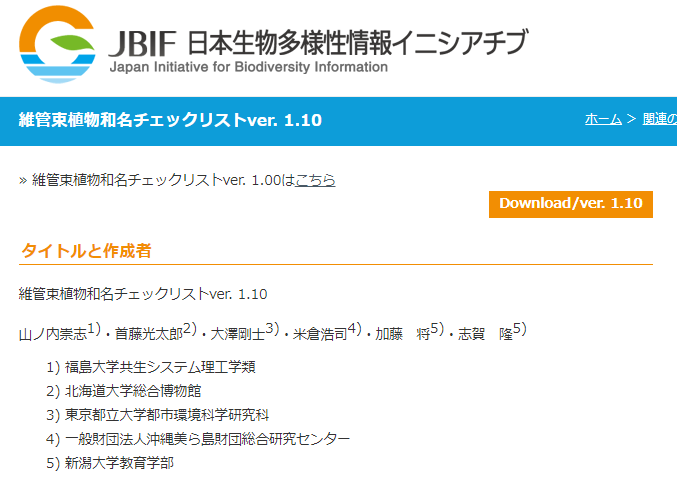
\includegraphics{image/wamei_web.png}

\newpage

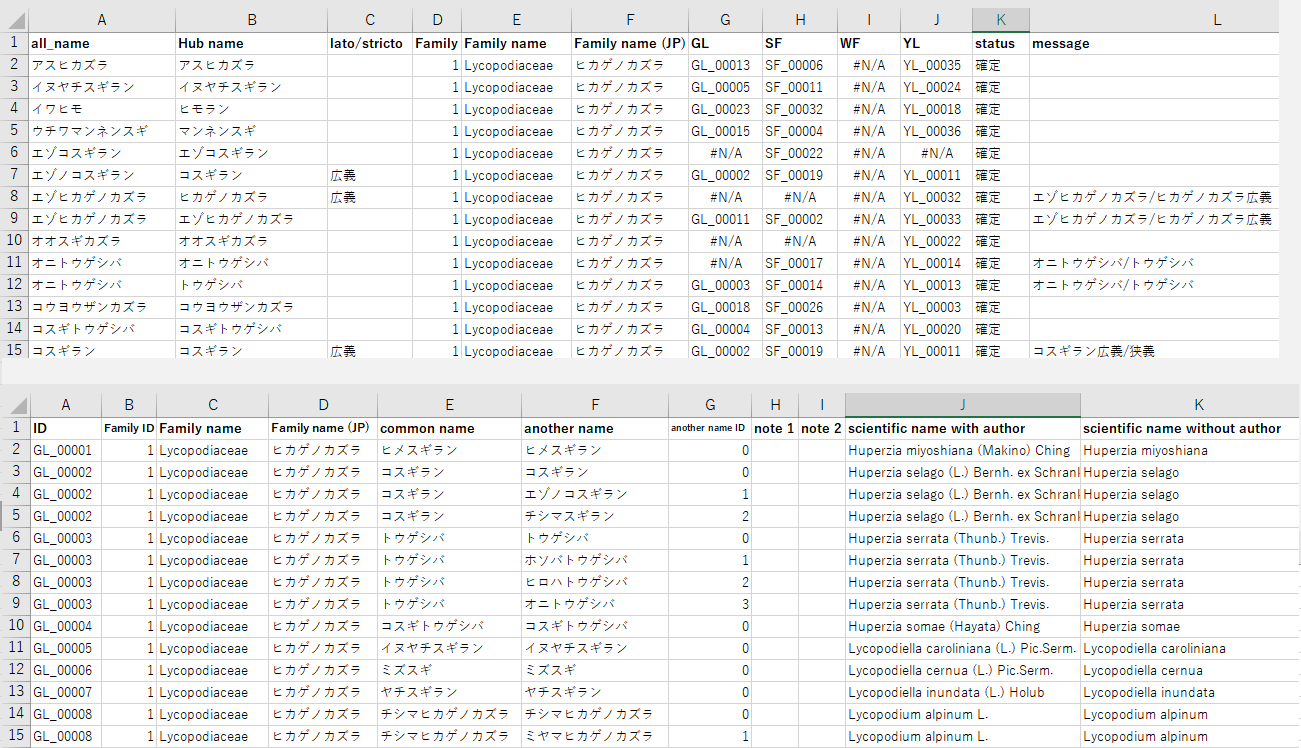
\includegraphics{image/wamei_hub_jn.png}

\newpage

\fontsize{32pt}{32pt}\selectfont

\begin{center}
維管束植物和名変換シート
\end{center}

\begin{itemize}
\tightlist
\item
  和名チェックリストを使いやすく\\
\item
  エクセル形式\\
\item
  手作業(コピペ)が必要\\
\item
  大量の場合は少し時間がかかる
\end{itemize}

\newpage

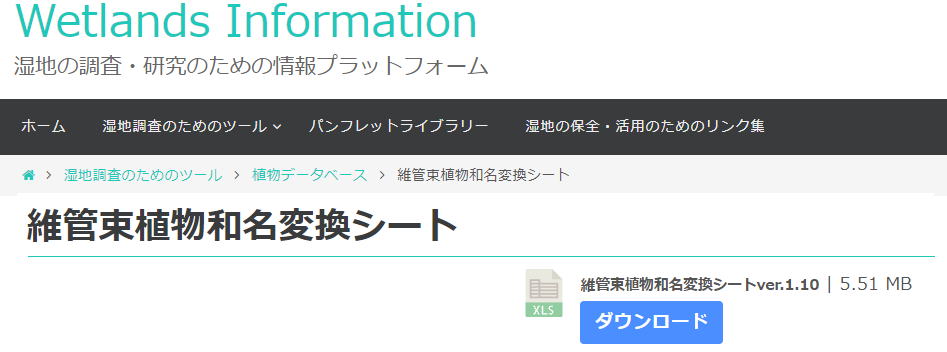
\includegraphics{image/convert_web.png}

\vspace{20pt}

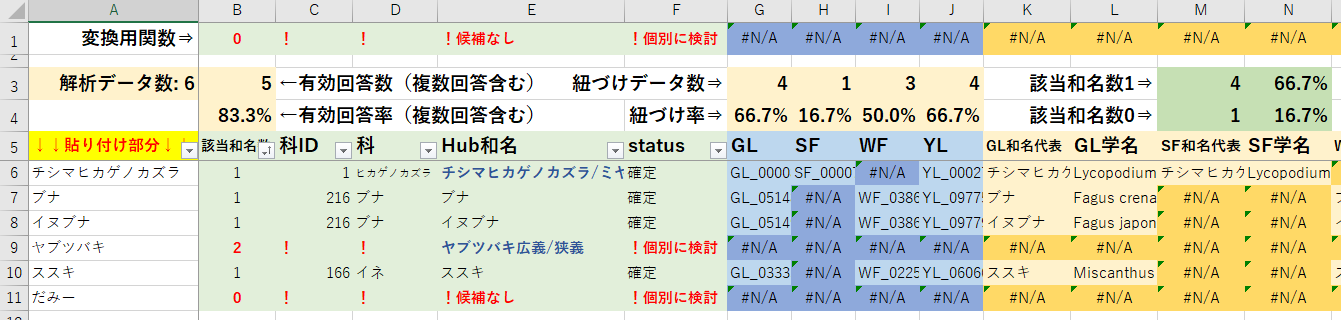
\includegraphics{image/convert_convert.png}

\newpage

\fontsize{32pt}{32pt}\selectfont

\begin{center}
解析手順の問題
\end{center}

\begin{itemize}
\item
  手作業による作業の中断\\
  -- エクセルに入力\\
  -- チェック・変換(手作業)\\
  -- データ保存(手作業)\\
  -- Rで解析
\item
  Rでできたら便利では?\\
  -- エクセルに入力(ここは仕方なし)\\
  -- Rでチェック・変換,解析
\item
  Rで関数を作ってしまおう!
\end{itemize}

\newpage

\fontsize{32pt}{32pt}\selectfont

\begin{center}
wameicheckrの特徴
\end{center}

\begin{itemize}
\tightlist
\item
  和名チェックリストのデータを含む\\
  -- 更新は元のデータに合わせて(予定)\\
\item
  簡単な操作(のはず)\\
\item
  GitHubで公開
\end{itemize}

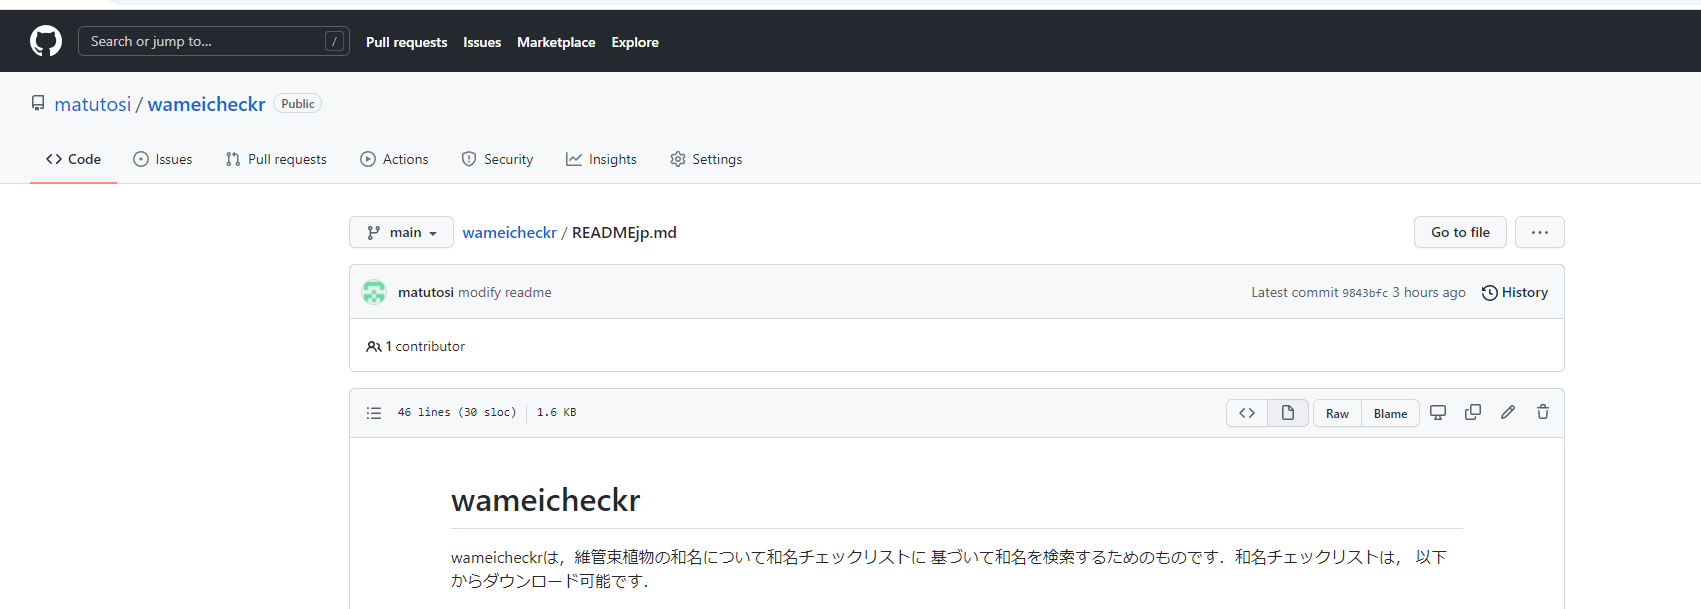
\includegraphics{image/wameicheckr.png}

\newpage

\fontsize{32pt}{32pt}\selectfont

\begin{center}
wameicheckrの使用方法
\end{center}

\begin{itemize}
\tightlist
\item
  インストール(省略)\\
\item
  準備・データ整理\\
\item
  元データのエラー修正\\
\item
  和名の準備\\
\item
  引数の説明\\
  -- 出力形式:横長 or 縦長\\
  -- データソース\\
\item
  関数による違い
\end{itemize}

\newpage

\fontsize{32pt}{32pt}\selectfont

\begin{center}
準備・データ整理
\end{center}

\fontsize{14pt}{14pt}\selectfont

\begin{Shaded}
\begin{Highlighting}[]
\FunctionTok{library}\NormalTok{(tidyverse)}
\FunctionTok{library}\NormalTok{(wameicheckr)}
\FunctionTok{library}\NormalTok{(magrittr)}
\end{Highlighting}
\end{Shaded}

\begin{Shaded}
\begin{Highlighting}[]
\FunctionTok{data}\NormalTok{(hub\_master)}
\FunctionTok{data}\NormalTok{(jn\_master)}

\NormalTok{hub\_master }\OtherTok{\textless{}{-}} 
\NormalTok{  hub\_master }\SpecialCharTok{\%\textgreater{}\%}
\NormalTok{  tibble}\SpecialCharTok{::}\FunctionTok{as\_tibble}\NormalTok{() }\SpecialCharTok{\%\textgreater{}\%}
\NormalTok{  dplyr}\SpecialCharTok{::}\FunctionTok{rename\_with}\NormalTok{(}\SpecialCharTok{\textasciitilde{}}\NormalTok{stringr}\SpecialCharTok{::}\FunctionTok{str\_replace\_all}\NormalTok{(., }\StringTok{"[ /]"}\NormalTok{, }\StringTok{"\_"}\NormalTok{)) }\SpecialCharTok{\%\textgreater{}\%}
\NormalTok{  dplyr}\SpecialCharTok{::}\FunctionTok{rename\_with}\NormalTok{(}\SpecialCharTok{\textasciitilde{}}\NormalTok{stringr}\SpecialCharTok{::}\FunctionTok{str\_replace\_all}\NormalTok{(., }\StringTok{"[()]"}\NormalTok{, }\StringTok{""}\NormalTok{)) }\SpecialCharTok{\%\textgreater{}\%}
  \FunctionTok{print}\NormalTok{(}\AttributeTok{n=}\DecValTok{5}\NormalTok{)}
\end{Highlighting}
\end{Shaded}

\begin{verbatim}
## # A tibble: 30,430 x 12
##   all_name     Hub_name  lato_stricto Family_ID Family_name Family_name_JP GL   
##   <chr>        <chr>     <chr>        <chr>     <chr>       <chr>          <chr>
## 1 アスヒカズラ アスヒカ~ <NA>         1         Lycopodiac~ ヒカゲノカズラ GL_0~
## 2 イヌヤチス~  イヌヤチ~ <NA>         1         Lycopodiac~ ヒカゲノカズラ GL_0~
## 3 イワヒモ     ヒモラン  <NA>         1         Lycopodiac~ ヒカゲノカズラ GL_0~
## 4 ウチワマン~  マンネン~ <NA>         1         Lycopodiac~ ヒカゲノカズラ GL_0~
## 5 エゾコスギ~  エゾコス~ <NA>         1         Lycopodiac~ ヒカゲノカズラ <NA> 
## # ... with 30,425 more rows, and 5 more variables: SF <chr>, WF <chr>,
## #   YL <chr>, status <chr>, message <chr>
\end{verbatim}

\newpage

\fontsize{32pt}{32pt}\selectfont

\begin{center}
準備・データ整理(続き)
\end{center}

\fontsize{14pt}{14pt}\selectfont

\begin{Shaded}
\begin{Highlighting}[]
\NormalTok{jn\_master }\OtherTok{\textless{}{-}} 
\NormalTok{  jn\_master }\SpecialCharTok{\%\textgreater{}\%}
\NormalTok{  tibble}\SpecialCharTok{::}\FunctionTok{as\_tibble}\NormalTok{() }\SpecialCharTok{\%\textgreater{}\%}
\NormalTok{  dplyr}\SpecialCharTok{::}\FunctionTok{rename\_with}\NormalTok{(}\SpecialCharTok{\textasciitilde{}}\NormalTok{stringr}\SpecialCharTok{::}\FunctionTok{str\_replace\_all}\NormalTok{(., }\StringTok{"[ /]"}\NormalTok{, }\StringTok{"\_"}\NormalTok{)) }\SpecialCharTok{\%\textgreater{}\%}
\NormalTok{  dplyr}\SpecialCharTok{::}\FunctionTok{rename\_with}\NormalTok{(}\SpecialCharTok{\textasciitilde{}}\NormalTok{stringr}\SpecialCharTok{::}\FunctionTok{str\_replace\_all}\NormalTok{(., }\StringTok{"[()]"}\NormalTok{, }\StringTok{""}\NormalTok{)) }\SpecialCharTok{\%\textgreater{}\%}
  \FunctionTok{fill\_another\_name\_id}\NormalTok{() }\SpecialCharTok{\%\textgreater{}\%} \CommentTok{\# another\_name\_id の空欄を埋める}
  \FunctionTok{print}\NormalTok{(}\AttributeTok{n=}\DecValTok{5}\NormalTok{)}
\end{Highlighting}
\end{Shaded}

\begin{verbatim}
## # A tibble: 53,222 x 11
##   ID       Family_ID Family_name   Family_name_JP common_name  another_name    
##   <chr>    <chr>     <chr>         <chr>          <chr>        <chr>           
## 1 GL_00001 1         Lycopodiaceae ヒカゲノカズラ ヒメスギラン ヒメスギラン    
## 2 GL_00002 1         Lycopodiaceae ヒカゲノカズラ コスギラン   コスギラン      
## 3 GL_00002 1         Lycopodiaceae ヒカゲノカズラ コスギラン   エゾノコスギラン
## 4 GL_00002 1         Lycopodiaceae ヒカゲノカズラ コスギラン   チシマスギラン  
## 5 GL_00003 1         Lycopodiaceae ヒカゲノカズラ トウゲシバ   トウゲシバ      
## # ... with 53,217 more rows, and 5 more variables: another_name_ID <dbl>,
## #   note_1 <chr>, note_2 <chr>, scientific_name_with_author <chr>,
## #   scientific_name_without_author <chr>
\end{verbatim}

\newpage

\fontsize{32pt}{32pt}\selectfont

\begin{center}
和名チェックリスト ver.1.10のエラーの修正   
バージョンアップで,修正される予定   
\end{center}

\fontsize{14pt}{14pt}\selectfont

\begin{Shaded}
\begin{Highlighting}[]
\NormalTok{no\_id\_0 }\OtherTok{\textless{}{-}} 
  \FunctionTok{c}\NormalTok{(}\StringTok{"SF\_00131"}\NormalTok{, }\StringTok{"SF\_00323"}\NormalTok{, }\StringTok{"WF\_01542"}\NormalTok{, }\StringTok{"WF\_02219"}\NormalTok{, }\StringTok{"WF\_04287"}\NormalTok{, }
  \StringTok{"SF\_00127"}\NormalTok{,}\StringTok{"WF\_01902"}\NormalTok{,}\StringTok{"WF\_03825"}\NormalTok{,}\StringTok{"YL\_11456"}\NormalTok{,}\StringTok{"YL\_17759"}\NormalTok{)}
\NormalTok{jn\_master}\SpecialCharTok{$}\NormalTok{another\_name\_ID[}
\NormalTok{  jn\_master}\SpecialCharTok{$}\NormalTok{ID }\SpecialCharTok{\%in\%}\NormalTok{ no\_id\_0 }\SpecialCharTok{\&}\NormalTok{ jn\_master}\SpecialCharTok{$}\NormalTok{another\_name\_ID }\SpecialCharTok{!=} \DecValTok{0}\NormalTok{] }\OtherTok{\textless{}{-}} \DecValTok{0}

  \CommentTok{\# (和名チェックリスト ver.1.10への対応) シベリアカラマツ(別科同名)}
\NormalTok{hub\_master}\SpecialCharTok{$}\NormalTok{Hub\_name[}
\NormalTok{  hub\_master}\SpecialCharTok{$}\NormalTok{Hub\_name}\SpecialCharTok{==}\StringTok{"シベリアカラマツ"} \SpecialCharTok{\&}\NormalTok{ hub\_master}\SpecialCharTok{$}\NormalTok{Family\_name\_JP}\SpecialCharTok{==}\StringTok{"マツ"}\NormalTok{] }\OtherTok{\textless{}{-}} 
  \StringTok{"シベリアカラマツ(マツ科)"}
\NormalTok{hub\_master}\SpecialCharTok{$}\NormalTok{Hub\_name[hub\_master}\SpecialCharTok{$}\NormalTok{Hub\_name}\SpecialCharTok{==}\StringTok{"シベリアカラマツ"} \SpecialCharTok{\&} 
\NormalTok{  hub\_master}\SpecialCharTok{$}\NormalTok{Family\_name\_JP}\SpecialCharTok{==}\StringTok{"キンポウゲ"}\NormalTok{] }\OtherTok{\textless{}{-}}  \StringTok{"シベリアカラマツ(キンポウゲ科)"}
\NormalTok{jn\_master}\SpecialCharTok{$}\NormalTok{Family\_name\_JP[jn\_master}\SpecialCharTok{$}\NormalTok{Family\_name\_JP}\SpecialCharTok{==}\StringTok{"ツルボラン"}\NormalTok{] }\OtherTok{\textless{}{-}} 
  \StringTok{"ワスレグサ"}
\end{Highlighting}
\end{Shaded}

\newpage

\fontsize{32pt}{32pt}\selectfont

\begin{center}
x1:データ内の全和名(の一部)   
x2:和名の例   
\end{center}

\fontsize{14pt}{14pt}\selectfont

\begin{Shaded}
\begin{Highlighting}[]
\NormalTok{x1 }\OtherTok{\textless{}{-}} 
  \FunctionTok{c}\NormalTok{(hub\_master}\SpecialCharTok{$}\NormalTok{all\_name, hub\_master}\SpecialCharTok{$}\NormalTok{Hub\_name, }
\NormalTok{  jn\_master}\SpecialCharTok{$}\NormalTok{common\_name, jn\_master}\SpecialCharTok{$}\NormalTok{another\_name) }\SpecialCharTok{\%\textgreater{}\%}
\NormalTok{  purrr}\SpecialCharTok{::}\FunctionTok{map}\NormalTok{(str\_split, }\StringTok{"/"}\NormalTok{) }\SpecialCharTok{\%\textgreater{}\%}
  \FunctionTok{unlist}\NormalTok{() }\SpecialCharTok{\%\textgreater{}\%} \FunctionTok{unique}\NormalTok{() }\SpecialCharTok{\%\textgreater{}\%} \FunctionTok{sort}\NormalTok{() }\SpecialCharTok{\%\textgreater{}\%}
  \FunctionTok{c}\NormalTok{(}\StringTok{"だみーの和名"}\NormalTok{, .) }\SpecialCharTok{\%\textgreater{}\%}
\NormalTok{  .[}\DecValTok{1}\SpecialCharTok{:}\DecValTok{30}\NormalTok{]}

\NormalTok{x2 }\OtherTok{\textless{}{-}} \FunctionTok{c}\NormalTok{(}\StringTok{"だみー"}\NormalTok{, }\StringTok{"ススキ"}\NormalTok{, }\StringTok{"チガヤ"}\NormalTok{,  }\StringTok{"ハリガネワラビ"}\NormalTok{, }\StringTok{"オミナエシ"}\NormalTok{, }
  \StringTok{"カナビキソウ"}\NormalTok{, }\StringTok{"ヤイトバナ"}\NormalTok{, }\StringTok{"キジムシロ"}\NormalTok{, }\StringTok{"ハエドクソウ"}\NormalTok{, }\StringTok{"コナスビ"}\NormalTok{, }
  \StringTok{"キツネノマゴ"}\NormalTok{, }\StringTok{"シロヨメナ"}\NormalTok{, }\StringTok{"オオフジシダ"}\NormalTok{, }\StringTok{"コマツナギ"}\NormalTok{, }
  \StringTok{"アイヌタチツボスミレ"}\NormalTok{, }\StringTok{"シベリアカラマツ"}\NormalTok{, }\StringTok{"アオイモドキ"}\NormalTok{)}
\end{Highlighting}
\end{Shaded}

\newpage

\fontsize{32pt}{32pt}\selectfont

\begin{center}
使用方法
\end{center}

\fontsize{22pt}{22pt}\selectfont

\begin{Shaded}
\begin{Highlighting}[]
\FunctionTok{wamei\_check}\NormalTok{(}
\NormalTok{  x,           }\CommentTok{\# 検索する和名}
\NormalTok{  hub\_master,  }\CommentTok{\# Hubデータ}
\NormalTok{  jn\_master,   }\CommentTok{\# jnデータ}
  \AttributeTok{wide =} \ConstantTok{TRUE}\NormalTok{, }\CommentTok{\# 出力形式(TRUE:横長,FALSE:縦長)}
  \AttributeTok{ds =} \FunctionTok{c}\NormalTok{(GL, SF, WF, YL)  }\CommentTok{\# データソース}
    \CommentTok{\# GL:Green List}
    \CommentTok{\# SF:シダ標準図鑑}
    \CommentTok{\# WF:日本の野生植物}
    \CommentTok{\# YL:Ylist}
\NormalTok{  )}
\end{Highlighting}
\end{Shaded}

\newpage

\fontsize{32pt}{32pt}\selectfont

\begin{center}
横長(上)と縦長(下)
\end{center}

\fontsize{12pt}{12pt}\selectfont

\begin{Shaded}
\begin{Highlighting}[]
\FunctionTok{wamei\_check}\NormalTok{(x1, hub\_master, jn\_master, }\AttributeTok{ds=}\FunctionTok{c}\NormalTok{(WF, YL)) }\SpecialCharTok{\%\textgreater{}\%} 
  \FunctionTok{select}\NormalTok{(input, }\SpecialCharTok{!}\FunctionTok{contains}\NormalTok{(}\StringTok{"Fami"}\NormalTok{) }\SpecialCharTok{\&} \FunctionTok{contains}\NormalTok{(}\FunctionTok{c}\NormalTok{(}\StringTok{"ID"}\NormalTok{, }\StringTok{"comm"}\NormalTok{))) }\SpecialCharTok{\%\textgreater{}\%} \FunctionTok{print}\NormalTok{(}\AttributeTok{n=}\DecValTok{5}\NormalTok{)}
\end{Highlighting}
\end{Shaded}

\begin{verbatim}
## # A tibble: 30 x 5
##   input         WF_ID    YL_ID    WF_common_name       YL_common_name      
##   <chr>         <chr>    <chr>    <chr>                <chr>               
## 1 だみーの和名  -        -        -                    -                   
## 2 mulberry      WF_03422 YL_09601 マグワ               マグワ              
## 3 no named      -        -        -                    -                   
## 4 no_named_GL01 -        -        -                    -                   
## 5 no_named_GL02 WF_00924 YL_03378 ムカゴサイシンモドキ ムカゴサイシンモドキ
## # ... with 25 more rows
\end{verbatim}

\begin{Shaded}
\begin{Highlighting}[]
\FunctionTok{wamei\_check}\NormalTok{(x1, hub\_master, jn\_master, }\AttributeTok{ds=}\FunctionTok{c}\NormalTok{(WF, YL), }\AttributeTok{wide=}\ConstantTok{FALSE}\NormalTok{) }\SpecialCharTok{\%\textgreater{}\%}
  \FunctionTok{select}\NormalTok{(input, source, ID, common\_name) }\SpecialCharTok{\%\textgreater{}\%} \FunctionTok{print}\NormalTok{(}\AttributeTok{n=}\DecValTok{7}\NormalTok{)}
\end{Highlighting}
\end{Shaded}

\begin{verbatim}
## # A tibble: 38 x 4
##   input         source ID       common_name         
##   <chr>         <chr>  <chr>    <chr>               
## 1 だみーの和名  -      -        -                   
## 2 mulberry      WF     WF_03422 マグワ              
## 3 mulberry      YL     YL_09601 マグワ              
## 4 no named      -      -        -                   
## 5 no_named_GL01 -      -        -                   
## 6 no_named_GL02 WF     WF_00924 ムカゴサイシンモドキ
## 7 no_named_GL02 YL     YL_03378 ムカゴサイシンモドキ
## # ... with 31 more rows
\end{verbatim}

\newpage

\fontsize{32pt}{32pt}\selectfont

\begin{center}
関数による違い
\end{center}

\fontsize{12pt}{12pt}\selectfont

\begin{Shaded}
\begin{Highlighting}[]
\FunctionTok{wamei\_check}\NormalTok{(x2, hub\_master, jn\_master, }\AttributeTok{wide=}\ConstantTok{FALSE}\NormalTok{) }\SpecialCharTok{\%\textgreater{}\%}
\NormalTok{  dplyr}\SpecialCharTok{::}\FunctionTok{select}\NormalTok{(input, status, source, ID, common\_name) }\SpecialCharTok{\%\textgreater{}\%} \FunctionTok{print}\NormalTok{(}\AttributeTok{n=}\DecValTok{8}\NormalTok{)}
\end{Highlighting}
\end{Shaded}

\begin{verbatim}
## # A tibble: 56 x 5
##   input  status   source ID       common_name
##   <chr>  <chr>    <chr>  <chr>    <chr>      
## 1 だみー 該当なし -      -        -          
## 2 ススキ 確定     GL     GL_03335 ススキ     
## 3 ススキ 確定     WF     WF_02250 ススキ     
## 4 ススキ 確定     YL     YL_06066 ススキ     
## 5 チガヤ 確定     YL     YL_05973 チガヤ     
## 6 チガヤ 確定     GL     GL_03283 チガヤ     
## 7 チガヤ 確定     WF     WF_02228 チガヤ     
## 8 チガヤ 確定     YL     YL_05974 チガヤ     
## # ... with 48 more rows
\end{verbatim}

\begin{Shaded}
\begin{Highlighting}[]
\FunctionTok{wamei\_check\_ex}\NormalTok{(x2, hub\_master, jn\_master, }\AttributeTok{wide=}\ConstantTok{FALSE}\NormalTok{) }\SpecialCharTok{\%\textgreater{}\%} 
\NormalTok{  dplyr}\SpecialCharTok{::}\FunctionTok{select}\NormalTok{(input, status, source, ID, common\_name) }\SpecialCharTok{\%\textgreater{}\%} \FunctionTok{print}\NormalTok{(}\AttributeTok{n=}\DecValTok{5}\NormalTok{)}
\end{Highlighting}
\end{Shaded}

\begin{verbatim}
## # A tibble: 27 x 5
##   input  status       source ID       common_name
##   <chr>  <chr>        <chr>  <chr>    <chr>      
## 1 だみー !個別に検討 <NA>   <NA>     <NA>       
## 2 ススキ 確定         GL     GL_03335 ススキ     
## 3 ススキ 確定         WF     WF_02250 ススキ     
## 4 ススキ 確定         YL     YL_06066 ススキ     
## 5 チガヤ !個別に検討 <NA>   <NA>     <NA>       
## # ... with 22 more rows
\end{verbatim}

\newpage

\fontsize{32pt}{32pt}\selectfont

\begin{center}
類似和名・学名検索(新機能)
\end{center}

\fontsize{24pt}{24pt}\selectfont

\begin{itemize}
\tightlist
\item
  文字列の編集距離\\
  -- 2つの文字列の近さを示す\\
  -- 挿入・置換・削除の手順の回数\\
  -- 例:ハッカグサとハシカグサの距離は1(1回の置換)\\
\item
  標準化した編集距離\\
  -- 編集距離 / 長い方の文字列の文字数
\item
  検索用の関数\\
  -- 一般:search\_similar\_name()\\
  -- 和名:mosiya()\\
  -- 学名:maybe()
\end{itemize}

\newpage

\fontsize{32pt}{32pt}\selectfont

\begin{center}
類似和名・学名の検索
\end{center}

\fontsize{16pt}{16pt}\selectfont

\begin{Shaded}
\begin{Highlighting}[]
\FunctionTok{data}\NormalTok{(ref\_jp)  }\CommentTok{\# 和名の参照用データ}
\NormalTok{ref\_jp        }\CommentTok{\# 和名は文字コードの関係でエスケープ文字を使用}
\end{Highlighting}
\end{Shaded}

\begin{verbatim}
## # A tibble: 51,809 x 2
##    source name_jp                                                   
##    <chr>  <chr>                                                     
##  1 GL     "\\u30d2\\u30e1\\u30b9\\u30ae\\u30e9\\u30f3"              
##  2 GL     "\\u30b3\\u30b9\\u30ae\\u30e9\\u30f3"                     
##  3 GL     "\\u30a8\\u30be\\u30ce\\u30b3\\u30b9\\u30ae\\u30e9\\u30f3"
##  4 GL     "\\u30c1\\u30b7\\u30de\\u30b9\\u30ae\\u30e9\\u30f3"       
##  5 GL     "\\u30c8\\u30a6\\u30b2\\u30b7\\u30d0"                     
##  6 GL     "\\u30db\\u30bd\\u30d0\\u30c8\\u30a6\\u30b2\\u30b7\\u30d0"
##  7 GL     "\\u30d2\\u30ed\\u30cf\\u30c8\\u30a6\\u30b2\\u30b7\\u30d0"
##  8 GL     "\\u30aa\\u30cb\\u30c8\\u30a6\\u30b2\\u30b7\\u30d0"       
##  9 GL     "\\u30b3\\u30b9\\u30ae\\u30c8\\u30a6\\u30b2\\u30b7\\u30d0"
## 10 GL     "\\u30a4\\u30cc\\u30e4\\u30c1\\u30b9\\u30ae\\u30e9\\u30f3"
## # ... with 51,799 more rows
\end{verbatim}

\newpage

\fontsize{32pt}{32pt}\selectfont

\begin{center}
類似和名・学名の検索
\end{center}

\fontsize{16pt}{16pt}\selectfont

\begin{Shaded}
\begin{Highlighting}[]
\FunctionTok{data}\NormalTok{(ref\_sc)  }\CommentTok{\# 学名の参照用データ}
\NormalTok{ref\_sc}
\end{Highlighting}
\end{Shaded}

\begin{verbatim}
## # A tibble: 76,379 x 2
##    source name_sc                                              
##    <chr>  <chr>                                                
##  1 GL     Huperzia miyoshiana (Makino) Ching                   
##  2 GL     Huperzia miyoshiana                                  
##  3 GL     Huperzia selago (L.) Bernh. ex Schrank et C.F.P.Mart.
##  4 GL     Huperzia selago                                      
##  5 GL     Huperzia serrata (Thunb.) Trevis.                    
##  6 GL     Huperzia serrata                                     
##  7 GL     Huperzia somae (Hayata) Ching                        
##  8 GL     Huperzia somae                                       
##  9 GL     Lycopodiella caroliniana (L.) Pic.Serm.              
## 10 GL     Lycopodiella caroliniana                             
## # ... with 76,369 more rows
\end{verbatim}

\newpage

\fontsize{32pt}{32pt}\selectfont

\begin{center}
類似和名の検索(1つだけ入力)
\end{center}

\fontsize{14pt}{14pt}\selectfont

\begin{Shaded}
\begin{Highlighting}[]
  \CommentTok{\# 和名: search\_similar\_name() では len=6 が必須(文字コードの関係)}
  \CommentTok{\# dist, dist\_normの小さい順で出力}
  \CommentTok{\# 既定値:min\_dist=4未満 or min\_dist\_norm=0.2未満を出力}
  \CommentTok{\# 対象文字列が短いと,編集距離4ではほとんど意味がない}
\FunctionTok{search\_similar\_name}\NormalTok{(}\StringTok{"ハッカグサ"}\NormalTok{, }\AttributeTok{len=}\DecValTok{6}\NormalTok{)}
\end{Highlighting}
\end{Shaded}

\begin{verbatim}
## # A tibble: 592 x 5
##    input      maybe                                        dist dist_norm source
##    <chr>      <chr>                                       <int>     <dbl> <chr> 
##  1 ハッカグサ スギナ                                          3     0.6   GL; S~
##  2 ハッカグサ トクサ                                          3     0.6   GL; S~
##  3 ハッカグサ コシダ                                          3     0.6   GL; S~
##  4 ハッカグサ メヘゴ                                          3     0.6   GL; S~
##  5 ハッカグサ ヘゴ                                            2     0.4   GL; S~
##  6 ハッカグサ オオアマクサシダ×リュウキュウイノモトソウ       4     0.190 GL; SF
##  7 ハッカグサ ワラビ                                          3     0.6   GL; S~
##  8 ハッカグサ ウスバミヤマノコギリシダ×ミヤマノコギリシダ     4     0.182 GL; SF
##  9 ハッカグサ ホソバノコギリシダ×ヒロハミヤマノコギリシダ     4     0.182 GL; SF
## 10 ハッカグサ ホソバノコギリシダ×オオバミヤマノコギリシダ     4     0.182 GL; SF
## # ... with 582 more rows
\end{verbatim}

\newpage

\fontsize{32pt}{32pt}\selectfont

\begin{center}
類似和名の検索(1つだけ入力)
\end{center}

\fontsize{14pt}{14pt}\selectfont

\begin{Shaded}
\begin{Highlighting}[]
  \CommentTok{\# 検索後にふるい分け}
\FunctionTok{search\_similar\_name}\NormalTok{(}\StringTok{"ハッカグサ"}\NormalTok{, }\AttributeTok{len=}\DecValTok{6}\NormalTok{) }\SpecialCharTok{\%\textgreater{}\%}
\NormalTok{  dplyr}\SpecialCharTok{::}\FunctionTok{filter}\NormalTok{(dist }\SpecialCharTok{\textless{}} \DecValTok{3} \SpecialCharTok{\&}\NormalTok{ dist\_norm }\SpecialCharTok{\textless{}} \FloatTok{0.5}\NormalTok{)}
\end{Highlighting}
\end{Shaded}

\begin{verbatim}
## # A tibble: 113 x 5
##    input      maybe  dist dist_norm source    
##    <chr>      <chr> <int>     <dbl> <chr>     
##  1 ハッカグサ ヘゴ      2       0.4 GL; SF; YL
##  2 ハッカグサ モミ      2       0.4 GL; WF; YL
##  3 ハッカグサ ツガ      2       0.4 GL; WF; YL
##  4 ハッカグサ ナギ      2       0.4 GL; WF; YL
##  5 ハッカグサ スギ      2       0.4 GL; WF; YL
##  6 ハッカグサ ネズ      2       0.4 GL; WF; YL
##  7 ハッカグサ ムロ      2       0.4 GL; WF; YL
##  8 ハッカグサ ヒデ      2       0.4 GL; WF; YL
##  9 ハッカグサ カヤ      2       0.4 GL; WF; YL
## 10 ハッカグサ クス      2       0.4 GL; YL    
## # ... with 103 more rows
\end{verbatim}

\newpage

\fontsize{32pt}{32pt}\selectfont

\begin{center}
類似学名の検索(1つだけ入力)
\end{center}

\fontsize{14pt}{14pt}\selectfont

\begin{Shaded}
\begin{Highlighting}[]
  \CommentTok{\# dist, dist\_normの小さい順で出力}
\FunctionTok{search\_similar\_name}\NormalTok{(}\StringTok{"Viola madahuricaa"}\NormalTok{, }\AttributeTok{len=}\DecValTok{1}\NormalTok{) }\SpecialCharTok{\%\textgreater{}\%}
\NormalTok{  dplyr}\SpecialCharTok{::}\FunctionTok{filter}\NormalTok{(dist }\SpecialCharTok{\textless{}} \DecValTok{4} \SpecialCharTok{\&}\NormalTok{ dist\_norm }\SpecialCharTok{\textless{}} \FloatTok{0.2}\NormalTok{)}
\end{Highlighting}
\end{Shaded}

\begin{verbatim}
## # A tibble: 1 x 5
##   input             maybe              dist dist_norm source
##   <chr>             <chr>             <int>     <dbl> <chr> 
## 1 Viola madahuricaa Viola mandshurica     3     0.176 YL
\end{verbatim}

\newpage

\fontsize{32pt}{32pt}\selectfont

\begin{center}
類似和名の検索(複数入力)
\end{center}

\fontsize{14pt}{14pt}\selectfont

\begin{Shaded}
\begin{Highlighting}[]
  \CommentTok{\# 和名}
\FunctionTok{mosiya}\NormalTok{(}\FunctionTok{c}\NormalTok{(}\StringTok{"ハッカグサ"}\NormalTok{, }\StringTok{"スズノエンドウ"}\NormalTok{))}
\end{Highlighting}
\end{Shaded}

\begin{verbatim}
## # A tibble: 24 x 5
##    input      maybe                                      dist dist_norm source   
##    <chr>      <chr>                                     <int>     <dbl> <chr>    
##  1 ハッカグサ オオアマクサシダ×リュウキュウイノモトソウ     4     0.190 GL; SF   
##  2 ハッカグサ ウスバミヤマノコギリシダ×ミヤマノコギリ~      4     0.182 GL; SF   
##  3 ハッカグサ ホソバノコギリシダ×ヒロハミヤマノコギリ~      4     0.182 GL; SF   
##  4 ハッカグサ ホソバノコギリシダ×オオバミヤマノコギリ~      4     0.182 GL; SF   
##  5 ハッカグサ ヒロハミヤマノコギリシダ×オオバミヤマノ~      4     0.16  GL; SF   
##  6 ハッカグサ ヒロハミヤマノコギリシダ×ミヤマノコギリ~      4     0.182 GL; SF   
##  7 ハッカグサ オオバミヤマノコギリシダ×ミヤマノコギリ~      4     0.182 GL; SF   
##  8 ハッカグサ ハダカグリ                                    2     0.4   GL; YL   
##  9 ハッカグサ ハシカグサ                                    1     0.2   GL; WF; ~
## 10 ハッカグサ ハッカ                                        2     0.4   GL; WF; ~
## # ... with 14 more rows
\end{verbatim}

\newpage

\fontsize{32pt}{32pt}\selectfont

\begin{center}
類似和名の検索(複数入力)
\end{center}

\fontsize{14pt}{14pt}\selectfont

\begin{Shaded}
\begin{Highlighting}[]
  \CommentTok{\# 検索条件の変更が可能}
  \CommentTok{\# min\_dist: 編集距離}
  \CommentTok{\# min\_dist\_norm: 標準化した編集距離}
\FunctionTok{mosiya}\NormalTok{(}\FunctionTok{c}\NormalTok{(}\StringTok{"ハッカグサ"}\NormalTok{, }\StringTok{"スズノエンドウ"}\NormalTok{), }\AttributeTok{min\_dist=}\DecValTok{2}\NormalTok{, }\AttributeTok{min\_dist\_norm=}\FloatTok{0.1}\NormalTok{)}
\end{Highlighting}
\end{Shaded}

\begin{verbatim}
## # A tibble: 2 x 5
##   input          maybe             dist dist_norm source    
##   <chr>          <chr>            <int>     <dbl> <chr>     
## 1 ハッカグサ     ハシカグサ           1     0.2   GL; WF; YL
## 2 スズノエンドウ スズメノエンドウ     1     0.125 GL; WF; YL
\end{verbatim}

\newpage

\fontsize{32pt}{32pt}\selectfont

\begin{center}
類似学名の検索(複数入力)
\end{center}

\fontsize{14pt}{14pt}\selectfont

\begin{Shaded}
\begin{Highlighting}[]
\FunctionTok{maybe}\NormalTok{(}\FunctionTok{c}\NormalTok{(}\StringTok{"Viola madahuricaa"}\NormalTok{, }\StringTok{"Carex nevarta"}\NormalTok{))}
\end{Highlighting}
\end{Shaded}

\begin{verbatim}
## # A tibble: 66,562 x 5
##    input             maybe                               dist dist_norm source  
##    <chr>             <chr>                              <int>     <dbl> <chr>   
##  1 Viola madahuricaa Huperzia miyoshiana (Makino) Ching     4    0.118  GL; SF;~
##  2 Viola madahuricaa Huperzia selago (L.) Bernh. ex Sc~     4    0.0755 GL; SF;~
##  3 Viola madahuricaa Huperzia serrata (Thunb.) Trevis.      4    0.121  GL; SF;~
##  4 Viola madahuricaa Huperzia somae (Hayata) Ching          4    0.138  GL; SF;~
##  5 Viola madahuricaa Lycopodiella caroliniana (L.) Pic~     4    0.103  GL; SF;~
##  6 Viola madahuricaa Lycopodiella caroliniana               4    0.167  GL; SF;~
##  7 Viola madahuricaa Lycopodiella cernua (L.) Pic.Serm.     4    0.118  GL; SF;~
##  8 Viola madahuricaa Lycopodiella inundata (L.) Holub       4    0.125  GL; SF;~
##  9 Viola madahuricaa Lycopodiella inundata                  4    0.190  GL; SF;~
## 10 Viola madahuricaa Lycopodium alpinum L.                  4    0.190  GL; SF;~
## # ... with 66,552 more rows
\end{verbatim}

\newpage

\fontsize{32pt}{32pt}\selectfont

\begin{center}
注意点・お願い
\end{center}

\begin{itemize}
\tightlist
\item
  Windows, Mac, Ubuntu で動くはず\\
\item
  和名チェックリストが更新中(修正中)\\
\item
  バグがあるかも:基本は自己責任で\\
\item
  要望やバグ報告は歓迎
\end{itemize}

\newpage

\fontsize{32pt}{32pt}\selectfont

\begin{center}
今後の方向性
\end{center}

\fontsize{22pt}{22pt}\selectfont

\begin{itemize}
\tightlist
\item
  search\_similar\_name()は汎用関数\\
  -- maybe(), mosiya()はsearch\_similar\_name()を使用\\
  -- 関数を改変すれば,他の分類群でも使用可能\\
  -- 自由に改変してください\\
  -- 方法不明の場合は連絡ください\\
\item
  維管束植物以外の日本産生物の種名の一覧\\
  -- \url{http://www.ujssb.org/checklist/index.html}\\
  --- wamei\_check() のような関数は要望があれば検討可能
\end{itemize}

\newpage

\fontsize{32pt}{32pt}\selectfont

\begin{center}
インストール方法
\end{center}

\fontsize{22pt}{22pt}\selectfont

\begin{Shaded}
\begin{Highlighting}[]
\FunctionTok{install.packages}\NormalTok{(}\StringTok{"devtools"}\NormalTok{)}
\NormalTok{devtools}\SpecialCharTok{::}\FunctionTok{install\_github}\NormalTok{(}\StringTok{"matutosi/wameicheckr"}\NormalTok{)}

\NormalTok{devtools}\SpecialCharTok{::}\FunctionTok{install\_github}\NormalTok{(}\StringTok{"matutosi/wameicheckr"}\NormalTok{,   }
  \AttributeTok{build\_vignettes =} \ConstantTok{TRUE}\NormalTok{) }\CommentTok{\# pandocが必要}
\end{Highlighting}
\end{Shaded}

\newpage

\fontsize{32pt}{32pt}\selectfont

\begin{center}
参考文献
\end{center}

\fontsize{20pt}{20pt}\selectfont

\begin{itemize}
\tightlist
\item
  Hadley Wickham (2016) Rパッケージ開発入門\\
  -- \url{https://r-pkgs.org/}\\
  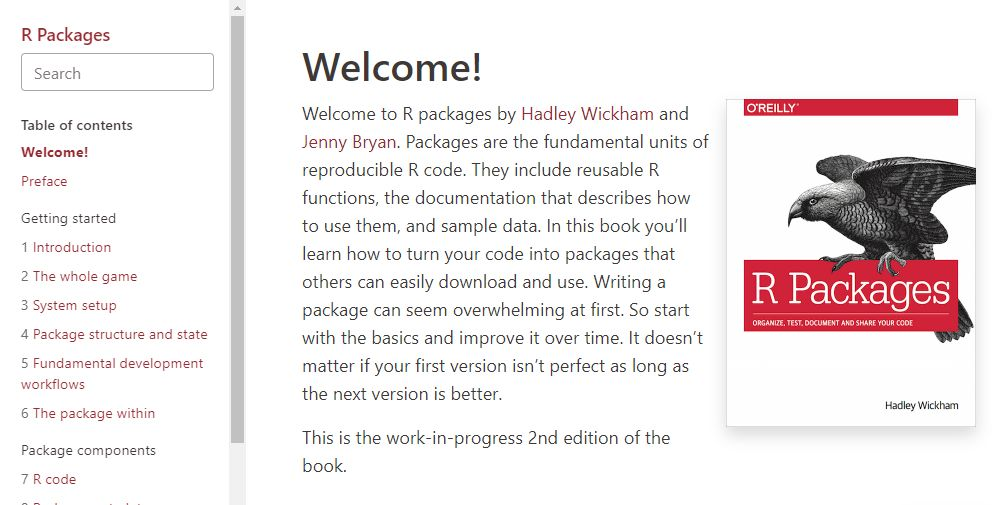
\includegraphics{image/r_packages_web.jpg}
\end{itemize}

\end{document}
